\subsection{Modelo conceptual}

\begin{figure}[H]
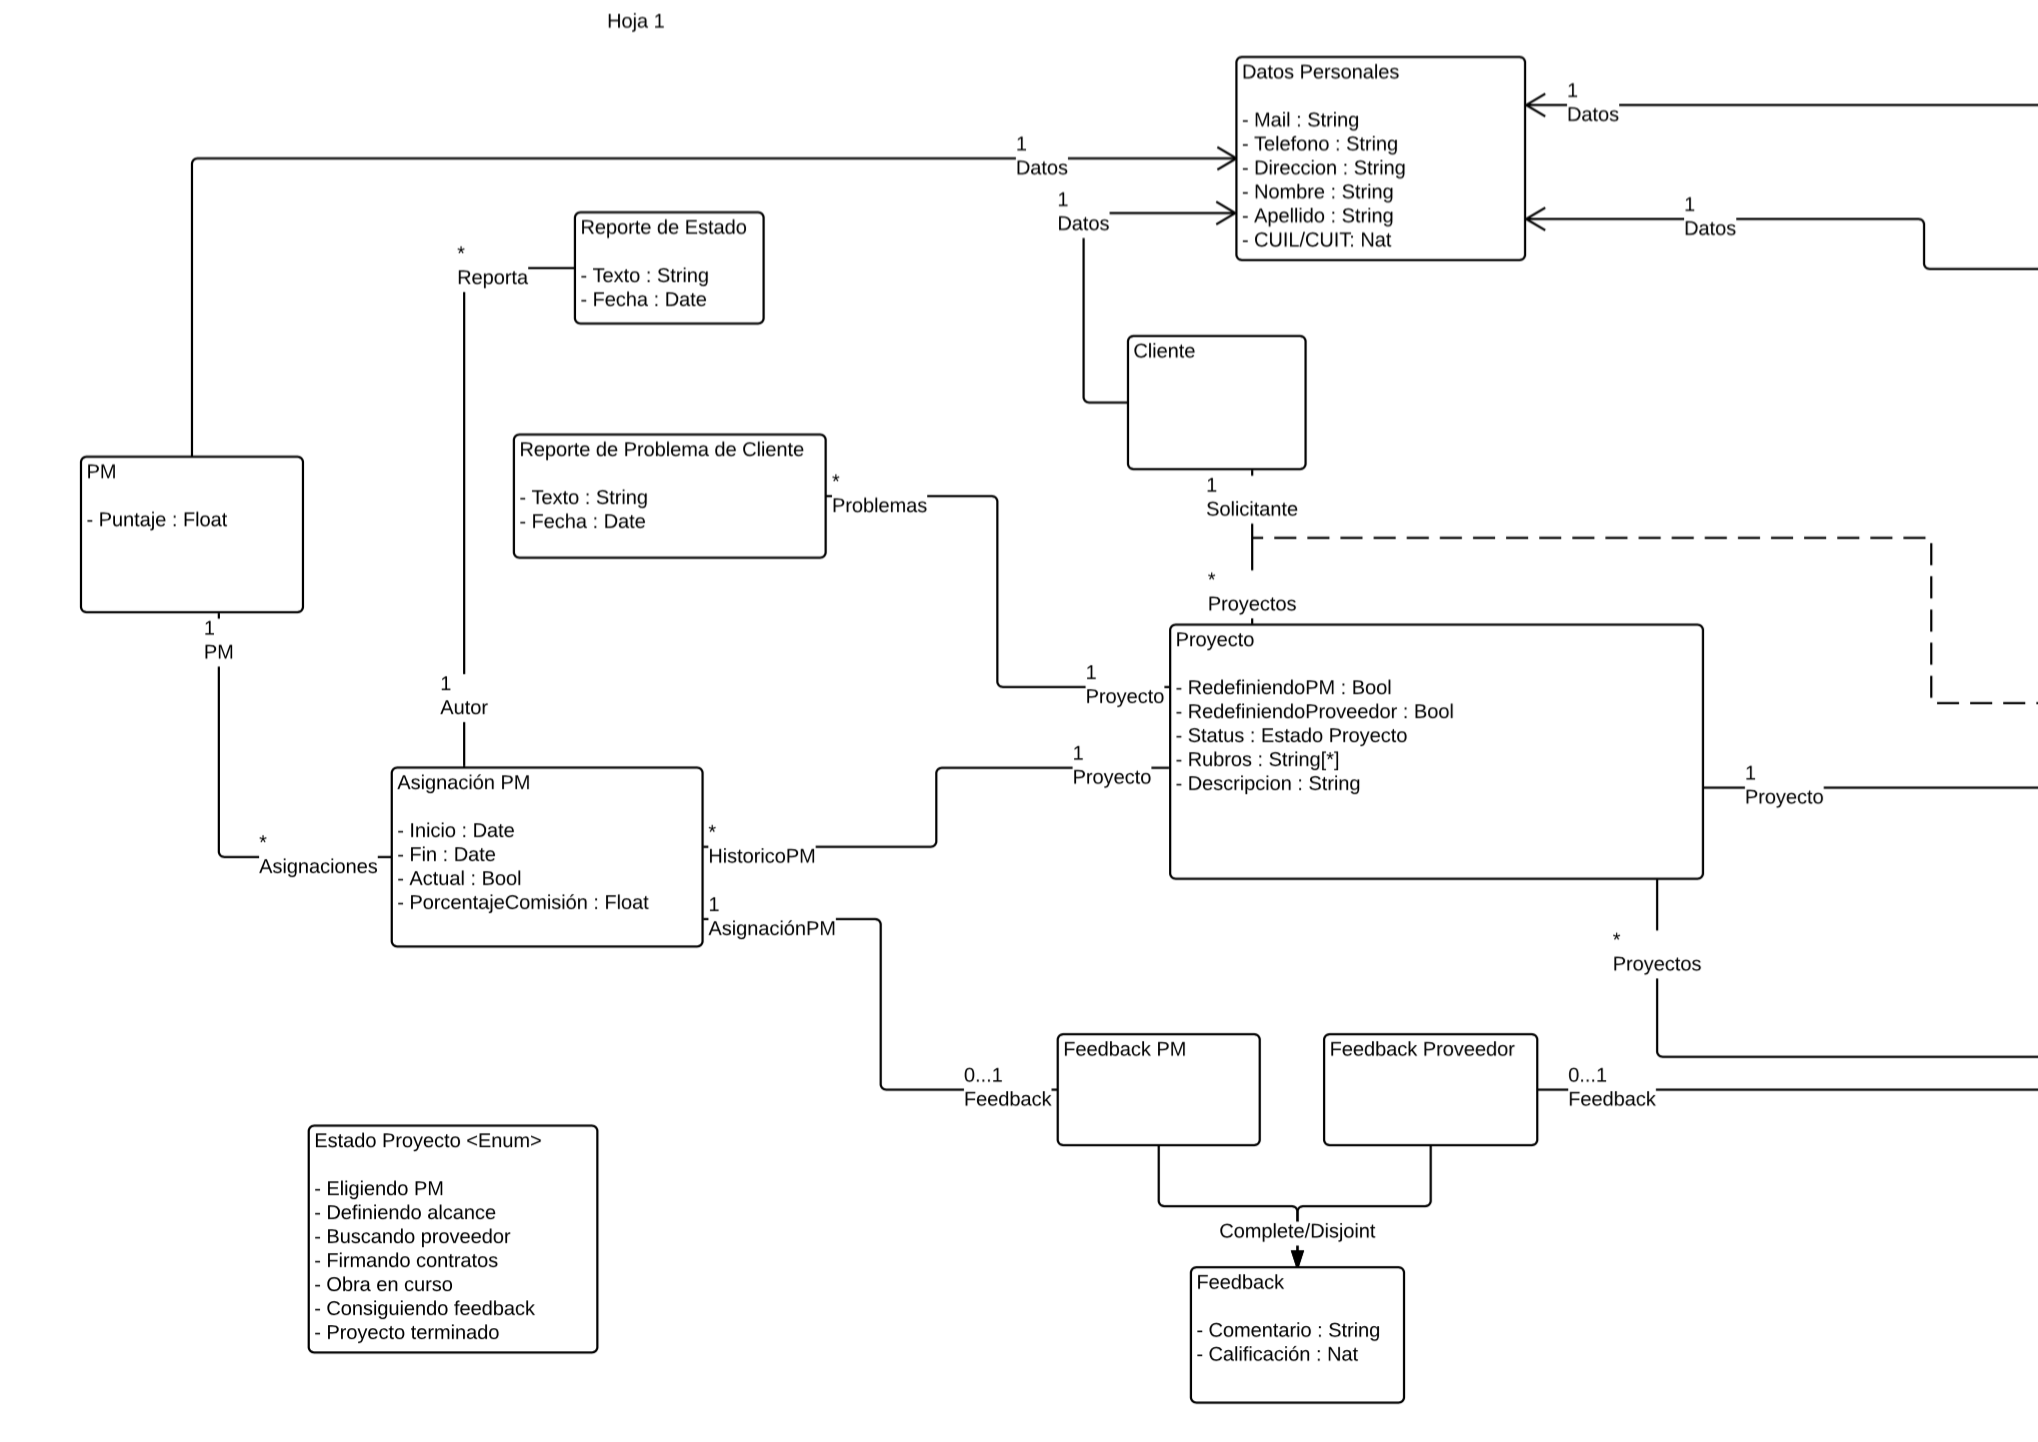
\includegraphics[width=\linewidth]{conc1.png}
\end{figure}
\begin{figure}[H]
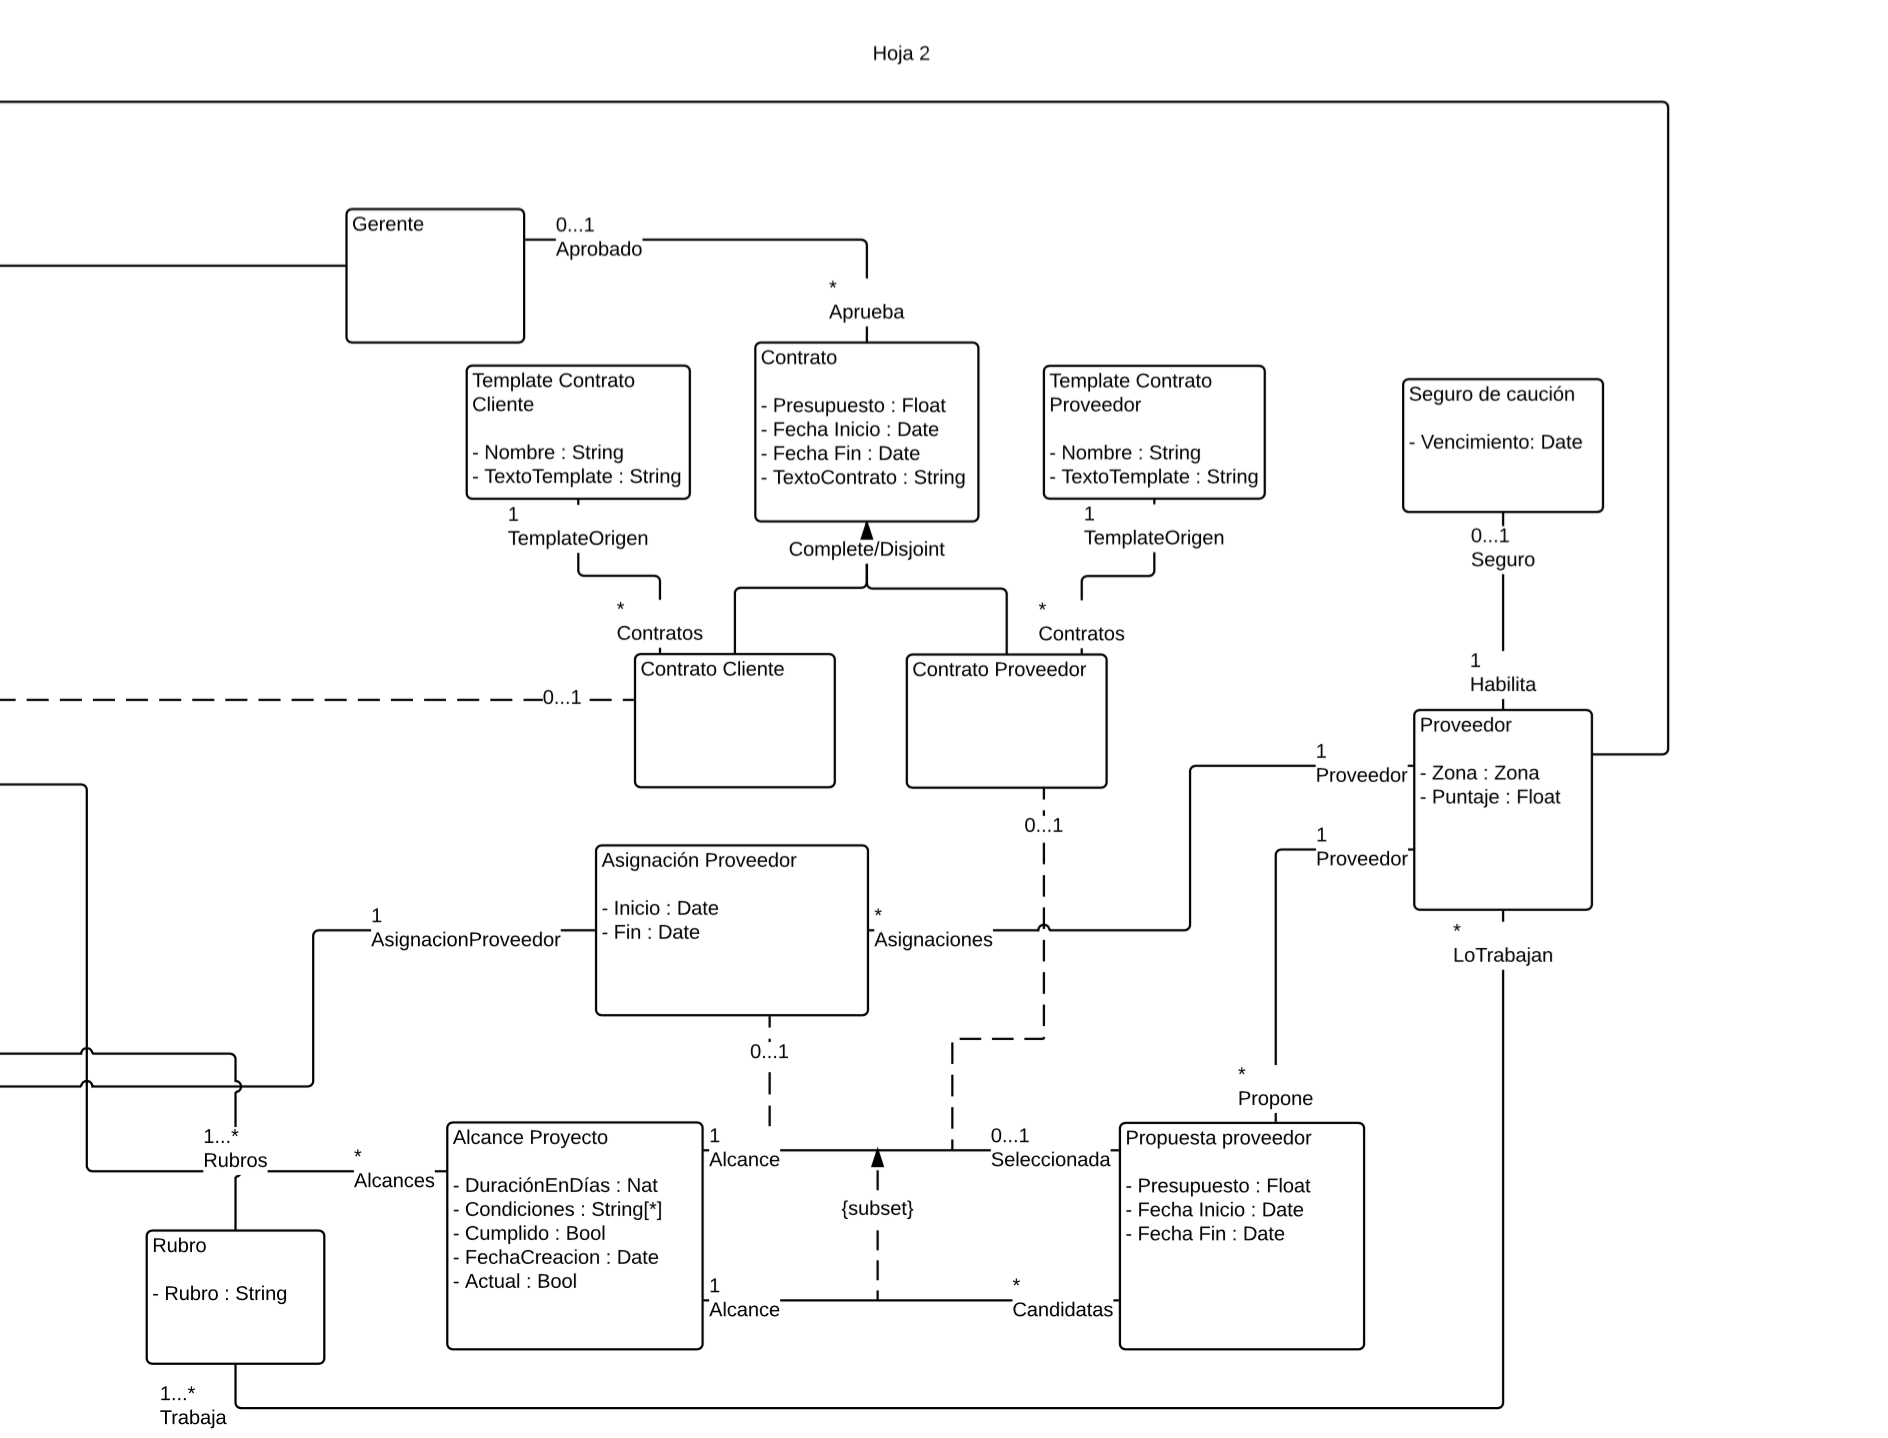
\includegraphics[width=\linewidth]{conc2.png}
\end{figure}

\subsubsection{Condiciones OCL}
\begin{itemize}
		\item	\textbf{Momentos en los cuales se puede redefinir el PM o proveedor de un proyecto:}
	
			Context: Proyecto
			
			\begin{tabular}{ll}
				self.redefiniendoProveedor $\Rightarrow$	& BuscandoProveedor < self.Status $\leq$ ObraEnCurso	\\
				self.redefiniendoPM $\Rightarrow$			& EligiendoPM < self.Status $\leq$ ObraEnCurso			\\
			\end{tabular}

	\item \textbf{Estado del proyecto:}

			Context: Proyecto
			
			\begin{tabular}{ll}
				\laterThan{EligiendoPM}				& \notEmpty{self.supervisaHistorico} and						\\
													& ((self.redefiniendoPM) xor (\notEmpty{self.supervisaActual}))	\\
				
				and \laterThan{DefiniendoAlcance}	& \notEmpty{self.alcance} \\
				
				and \laterThan{BuscandoProveedor}	& \notEmpty{self.proveedorHistorico} and	\\
													& (self.redefiniendoProveedor xor			\\
													& (\notEmpty{self.proveedorActual}))		\\
				
				and \laterThan{FirmandoContratos}	& \notEmpty{contratoCliente(self, self.Solicitante)} and	\\
													& (self.redefiniendoProveedor xor							\\
													& \notEmpty{contratoProveedor(self, self.ProveedorActual)})	\\
				
				and \laterThan{ConsiguiendoFeedback}	& \notEmpty{self.FeedbackProveedor} and	\\
														& \notEmpty{self.FeedbackPM}			\\
			\end{tabular}
			
	\item \textbf{Seguro de caución al día para proyectos actuales:}
	
			Context: Alcance Proyecto
			
			(self.Actual and self.Proyecto.Status $\in$ [BuscandoProveedor, obraEnCurso]	\\
			and \notEmpty{self.PropuestaProveedor.contratoProveedor}) 		\\
			$\Rightarrow$ (\notEmpty{self.Proveedor.Seguro} and self.Proveedor.Seguro.Vencimiento	\\
			> self.PropuestaProveedor.contratoProveedor.FechaFin)	\\
			
	\item \textbf{Los autores de reportes son PM del proyecto:}
		
			Context: Reporte de estado 
			
			\notEmpty{self.Autor.SupervisaHistorico $\rightarrow$ filter(p | p == self.Proyecto)}
	
	\item \textbf{Los puntajes de los agentes se corresponden con los puntajes seg\'un proyectos:}
			
			Context: PM
			
			\begin{tabular}{ll}
			self.puntaje ==	& self.Asignaciones\applyParam{filter}{Proyecto} \applyParam{select}{p$\|$\notEmpty{p.FeedbackPM}}	\\
							& \applyParam{filter}{FeedbackPM}\applyParam{filter}{Calificacion}\apply{average}	\\
			\end{tabular}
			
			Context: Proveedor
			
			\begin{tabular}{ll}
			self.puntaje ==	& self.Asignaciones\applyParam{select}{p$\|$\notEmpty{p.FeedbackProv}}\applyParam{filter}{FeedbackProv} \\
							& \applyParam{filter}{Calificacion}\apply{average}	\\
			\end{tabular}
	
	\item \textbf{Las asignaciones no se pisan en tiempo}
	
			Context: Proyecto
			
			self.Alcances\applyParam{filter}{AsignacionProveedor}\applyParam{forAll}{a1 $\neq$ a2$\|$a1.Inicio > a2.Fin or a2.Inicio > a1.Fin}
	
	\item \textbf{Hay a lo sumo un alcance actual y una asignación de PM actual}
	
			Context: Proyecto
			
			self.Alcances\applyParam{select}{a$\|$a.Actual}\apply{size} $\leq$ 1
			
			self.HistoricoPM\applyParam{select}{a$\|$a.Actual}\apply{size} $\leq$ 1
			
	\item \textbf{Ciclo Proveedor - Asignaci\'on - Propuesta}
	
			Context: Asignación Proveedor
			
			self.Proveedor == self.PropuestaProveedor.Proveedor
	
	%\item \textbf{Los estados del proyecto pero para el otro lado?}
	%\item \textbf{Fechas de los reportes?}
	%\item \textbf{Solapamiento de PMs historico}
	%\item \textbf{Solapamiento de proveedores historico?}
	%\item \textbf{Porcentaje de las comisiones}
	%\item \textbf{Fechas de fin luego de fechas de inicio}
	
        \item \textbf{Hay a lo sumo un alcance actual y una asignación de PM actual}
    
            Context: Proyecto
            
            self.Alcances\applyParam{select}{A$\|$a.Actual}\apply{size} $\leq$ 1
            
            self.HistoricoPM\applyParam{select}{A$\|$a.Actual}\apply{size} $\leq$ 1
    
    \item \textbf{Ciclo Proveedor - Propuesta - Asignacion}
    
            Context: Asignación Proveedor
            
            self.Proveedor == self.PropuestaProveedor.Proveedor
        
\end{itemize}
